% directive: erasureCodeStreamingFigure
% aria-label: Erasure-code streaming: the encoder emits chunks c_t = EncodePayload(y, t) at indices t mod N, here N = 8; chunks c_4 and c_7 are lost; the decoder adds the others and stores their distinct indices P = {0, 1, 2, 3, 5, 6}; Decode returns y if |P| >= k and bottom if |P| < k.
\documentclass[tikz,border=6pt]{standalone}
\usepackage[T1]{fontenc}
\usepackage{amsmath,amssymb}
\renewcommand{\familydefault}{\sfdefault}
\usepackage[eulergreek]{sansmath}
\sansmath
\usepackage{xcolor}
\usepackage{tikz}
\usetikzlibrary{positioning,calc,arrows.meta,fit,backgrounds,decorations.pathreplacing}
\definecolor{commentcolor}{HTML}{666666}
\definecolor{signalblue}{HTML}{3A76F0}
\definecolor{signalgreen}{HTML}{2A7B7B}
\definecolor{signalolive}{HTML}{4E7F60}
\definecolor{signalpurple}{HTML}{6B3FA0}
\definecolor{adversaryred}{HTML}{B42318}
\newcommand{\Encode}{\mathsf{Encode}}
\newcommand{\Decode}{\mathsf{Decode}}
\tikzset{
  panel/.style={draw=gray!45, line width=0.5pt, rounded corners=4pt, fill=gray!3, inner sep=6pt},
  algbox/.style={draw=signalolive!80, line width=0.7pt, rounded corners=3pt, fill=signalolive!10,
    inner sep=6pt, font=\small\sffamily, align=center},
  statebox/.style={draw=signalblue!70, line width=0.65pt, rounded corners=4pt, fill=signalblue!6,
    inner sep=6pt, font=\small\sffamily, align=center},
  keypill/.style={draw=signalpurple!75, line width=0.6pt, rounded corners=7pt, fill=signalpurple!9,
    inner xsep=8pt, inner ysep=4pt, font=\small\sffamily},
  chunk/.style={draw=signalblue!75, line width=0.55pt, rounded corners=2pt, fill=signalblue!9,
    minimum width=0.62cm, minimum height=0.50cm, inner sep=1pt, font=\scriptsize\sffamily},
  chunklost/.style={chunk, draw=gray!45, fill=gray!10, text=gray!55},
  sourcechunk/.style={chunk, draw=signalpurple!70, fill=signalpurple!9},
  goodpill/.style={draw=signalgreen!80, line width=0.65pt, rounded corners=7pt, fill=signalgreen!9,
    inner xsep=8pt, inner ysep=4pt, font=\small\sffamily},
  failpill/.style={draw=adversaryred!75, line width=0.65pt, rounded corners=7pt, fill=adversaryred!7,
    inner xsep=8pt, inner ysep=4pt, font=\small\sffamily},
  flow/.style={->, >=Stealth, line width=0.8pt, black},
  lossy/.style={->, >=Stealth, line width=0.5pt, gray!55, dashed},
  slot/.style={draw=gray!60, line width=0.5pt, minimum width=0.42cm, minimum height=0.42cm, inner sep=0pt},
  slotfull/.style={slot, fill=signalgreen!25, draw=signalgreen!70},
  slotempty/.style={slot, fill=white},
  lbl/.style={font=\small\sffamily, inner sep=2pt},
  slbl/.style={font=\scriptsize\sffamily, inner sep=1.5pt},
  note/.style={font=\scriptsize\sffamily\itshape, text=commentcolor, inner sep=1.5pt},
  theorybox/.style={draw=signalgreen!80, line width=0.8pt, rounded corners=4pt, fill=signalgreen!8,
    inner sep=7pt, font=\small\sffamily, align=center},
  instancebox/.style={draw=signalblue!70, line width=0.7pt, rounded corners=4pt, fill=signalblue!6,
    inner sep=7pt, font=\small\sffamily, align=center},
  instof/.style={->, >=Stealth, line width=0.8pt, black},
  uses/.style={->, >=Stealth, line width=0.7pt, dashed, signalolive},
  ecbox/.style={draw=signalblue!70, line width=0.7pt, rounded corners=3pt, fill=signalblue!7,
    inner sep=6pt, font=\small\sffamily, align=center},
  rolepill/.style={fill=signalgreen, text=white, rounded corners=5pt, inner xsep=9pt, inner ysep=4pt,
    font=\sffamily\bfseries},
  advpill/.style={draw=adversaryred!80, line width=0.7pt, rounded corners=5pt, fill=adversaryred!7,
    text=adversaryred, minimum width=1.05cm, minimum height=0.68cm, inner sep=3pt, font=\normalsize},
  timeline/.style={-, line width=0.6pt, gray!55},
}
\newcommand{\tagsf}[1]{{\scriptsize\sffamily\itshape\textcolor{commentcolor}{#1}}}
\newcommand{\notesf}[1]{{\scriptsize\sffamily\itshape\textcolor{signalpurple}{#1}}}

\tikzset{schunk/.style={draw=signalolive!70, line width=0.5pt, rounded corners=1pt, fill=white,
  minimum width=0.5cm, minimum height=0.42cm, inner sep=0pt, font=\scriptsize\sffamily},
  schunklost/.style={schunk, fill=gray!12, draw=gray!45, text=gray!55}}
\begin{document}
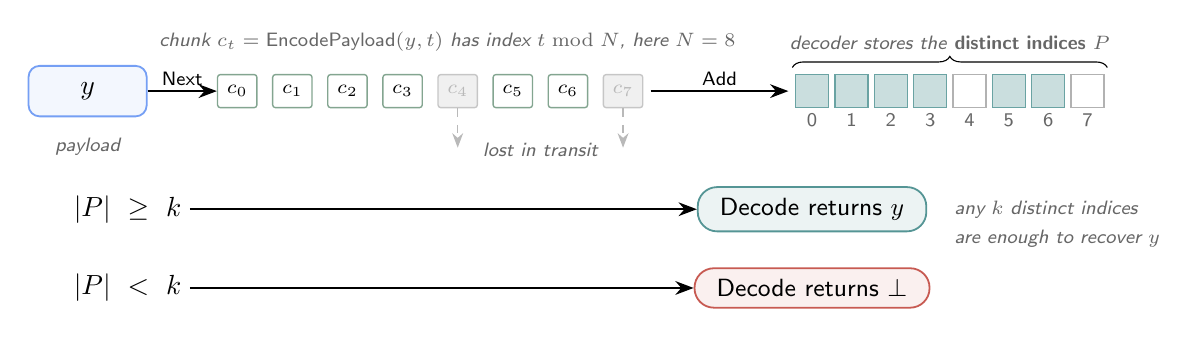
\begin{tikzpicture}[x=1cm, y=1cm]
  \node[statebox, minimum width=1.5cm, font=\normalsize] at (-6.6, 1.15) (M) {$y$};
  \node[note, anchor=north, align=center] at (-6.6, 0.62) {payload};
  \foreach \i/\x in {0/-4.7, 1/-4.0, 2/-3.3, 3/-2.6, 5/-1.2, 6/-0.5} {
    \node[schunk] at (\x, 1.15) (ch\i) {$c_{\i}$};
  }
  \node[schunklost] at (-1.9, 1.15) (ch4) {$c_4$};
  \node[schunklost] at ( 0.2, 1.15) (ch7) {$c_7$};
  \draw[flow] (M.east) -- node[above, slbl] {$\mathsf{Next}$} (ch0.west);
  \draw[lossy] (ch4.south) -- ++(0,-0.5);
  \draw[lossy] (ch7.south) -- ++(0,-0.5);
  \node[note, anchor=north] at (-0.85, 0.55) {lost in transit};
  \node[note, anchor=west] at (-5.75, 1.78)
    {chunk $c_t=\mathsf{EncodePayload}(y,t)$ has index $t \bmod N$, here $N=8$};
  \node[note, anchor=south, align=center] at (4.35, 1.62)
    {decoder stores the \textbf{distinct indices} $P$};
  \foreach \k in {0, 1, 2, 3, 5, 6} { \node[slotfull] at ({2.6 + 0.5*\k}, 1.15) {}; }
  \foreach \k in {4, 7} { \node[slotempty] at ({2.6 + 0.5*\k}, 1.15) {}; }
  \foreach \k in {0, ..., 7} { \node[slbl, text=commentcolor] at ({2.6 + 0.5*\k}, 0.78) {\k}; }
  \draw[decorate, decoration={brace, amplitude=4pt}] (2.35, 1.45) -- (6.35, 1.45);
  \draw[flow] (0.55, 1.15) -- node[above, slbl] {$\mathsf{Add}$} (2.3, 1.15);
  \node[goodpill] at (2.6, -0.35) (ok) {$\mathsf{Decode}$ returns $y$};
  \node[failpill] at (2.6, -1.35) (no) {$\mathsf{Decode}$ returns $\bot$};
  \node[anchor=west, font=\normalsize] at (-6.9, -0.35) {$|P| \ \ge\ k$};
  \node[anchor=west, font=\normalsize] at (-6.9, -1.35) {$|P| \ <\ k$};
  \draw[flow] (-5.3, -0.35) -- (ok.west);
  \draw[flow] (-5.3, -1.35) -- (no.west);
  \node[note, anchor=west, align=left] at (4.35, -0.35) {any $k$ distinct indices};
  \node[note, anchor=west, align=left] at (4.35, -0.72) {are enough to recover $y$};
\end{tikzpicture}
\end{document}
